\subsection{Vai trò từng thành phần và lựa chọn tham số}\label{sec:component-roles}
Hai lớp privacy đưa ra hai cận cho cùng transcript, không là hai con số ngân sách cộng trực tiếp.
Geo-I cung cấp profile theo khoảng cách trajectory và một nguồn thông tin đã bảo vệ cho belief.
Kernel Q giới hạn riêng sự phụ thuộc của hành động công khai vào thông tin riêng, kể cả khi belief
xấp xỉ. Belief là cơ chế thích nghi utility; nó không phải điều kiện để cận Q tồn tại.

Với cận toàn thời lượng đang dùng, điểm giao của hai envelope thô là
\begin{equation}
d_{\rm cross}=\frac{\log R_\infty^{\rm ub}}{C_s}
\simeq\frac{\log(2{,}437372)}{0{,}23}=3{,}874\text{ m}.
\label{eq:bound-crossing}
\end{equation}
Vì vậy ở thang so sánh hàng chục/hàng trăm mét, cận Q đang nhỏ hơn cận Geo-I thô. Điều này không
phủ định cận không gian, nhưng ngăn việc quy toàn bộ mức bảo vệ định lượng cho Geo-I. Cận envelope
tinh hơn $G_M$ có thể cải thiện riêng một cặp trajectories; hình không mô tả lượng tiết lộ thực đo.
\begin{figure}[htbp]\centering
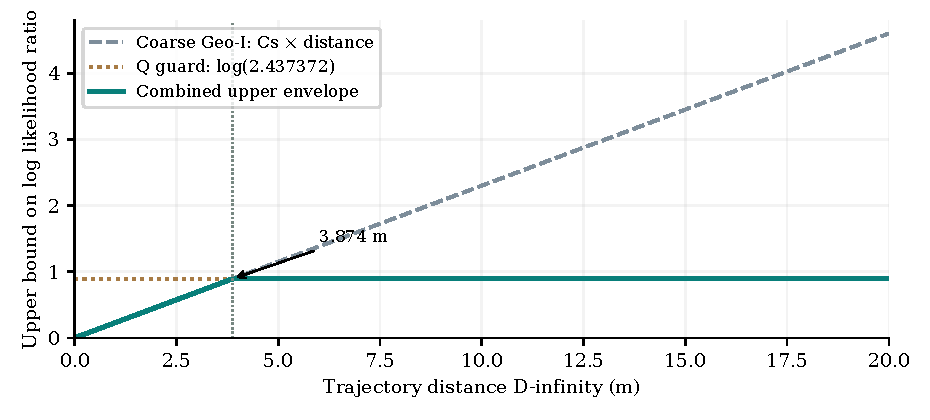
\includegraphics[width=.88\linewidth]{figures/privacy_bound_profile_20261116.pdf}
\caption{Profile của hai cận trên log-likelihood ratio, với cấu hình tham chiếu.
Đường minimum là cận lý thuyết, không là đường accuracy của attacker.}
\label{fig:bound-profile}
\end{figure}

\begin{center}\small
\begin{tabularx}{\linewidth}{@{}P{3.1cm}YY@{}}\toprule
Thành phần & Điều được phân tích & Điều chưa được suy ra\\\midrule
REM/noisy reuse/cap & Geo-I không gian của history lý tưởng; kiểm soát private reads &
Cap 0,23 không tự là lựa chọn tối ưu hoặc một bán kính nhiễu.\\
Belief & Proxy tính score từ protected history &
Bayes update gần đúng không chứng nhận calibration hoặc actual Recall gain.\\
Q kernel/ledger & Cận một đoạn, composition và hậu xử lý các khung &
Không cần claim mọi giá trị $\Gamma_Q>0$ tốt hơn public base.\\
Public retrieval/cache & Phủ ứng viên và local ranking đúng trên metadata hợp lệ &
Coverage cao không chứng minh cần private adaptation hoặc cần online query khi catalogue đã có.\\\bottomrule
\end{tabularx}
\end{center}

Một cách đặt yêu cầu trước khi thực nghiệm là chọn tỷ số cho phép $R_*>1$. Điều kiện đủ cho riêng
guard Q là $\Gamma_Q\le\log R_*$ vì $R_n\le e^{\Gamma_Q}$. Nếu yêu cầu riêng nhánh Geo-I tại độ
lệch $d_*$, dùng $C_s\le\log R_*/d_*$. Sau đó chọn $u,M$, lịch allowance và kiểm tra utility/cost
trên dữ liệu đã chốt. Đây là quy tắc thiết kế tổng quát; không hồi tố rằng cấu hình tham chiếu đã
được chọn bằng chính sách rủi ro này, hoặc tìm cấu hình có score TEST cao nhất rồi gọi nó là tối ưu.
